\documentclass[12pt]{article}
\usepackage[T1]{fontenc}
\usepackage{lmodern}
\usepackage[utf8]{inputenc}
\usepackage[margin=1in]{geometry}
\usepackage{graphicx}
\graphicspath{ {./screeny/} }
\usepackage{subfig}
\usepackage{float}
\usepackage{booktabs}
\usepackage[english, polish]{babel}
\usepackage{dirtytalk}
\usepackage{blindtext}
\usepackage{xcolor}
\usepackage{dirtree}
\usepackage{svg}

\usepackage{caption}
\captionsetup[figure]{labelformat=empty}

\usepackage{hyperref}

\hypersetup{
    colorlinks,
    citecolor=black,
    filecolor=magenta,
    linkcolor=blue,
    urlcolor=blue
}

\setlength{\parskip}{\baselineskip}

\setlength\parindent{0pt}
%\setlength\parskip{10pt}

\newcommand{\ttbf}[1]{
    \texttt{\textbf{#1}}
}

\newenvironment{console1}
{
    \ttfamily
    \fontseries{b}
    \selectfont
    {[}user@linux $\sim${]}\$} {

    }

\newenvironment{bv}{
    \ttfamily
    \fontseries{b}
    \selectfont
    \begin{verbatim}
        
}{\end{verbatim}}

\title{Obsługa terminalu dla opornych}
\author{Xerun\#0773}
\date{\today}

\begin{document}

\begin{titlepage}
    \null  % Empty line
    \nointerlineskip  % No skip for prev line
    \vfill
    \let\snewpage \newpage
    \let\newpage \relax
    \maketitle
    \let \newpage \snewpage
    \vfill 
    \break % page break
\end{titlepage}

\section*{O czym jest ten dokument?}
    W tym dokumencie postaram się w sposób przystępny przekazać tajniki działania terminala w systemie Linux. Pokażę, że nie jest to nic strasznego i nie trzeba się tego bać. Terminal jest bardzo przydatnym narzędziem, które tylko wygląda nieprzystępnie. Dodatkowo ten dokument może funkcjonować jako baza wiedzy o pewnych komendach i ich prostych przykładach, do której można zajrzeć w dowolnym momencie. Dla ułatwienia takiego użytkowania można skorzystać ze spisu treści, którego elementy po kliknięciu powinny zaprowadzić Cię do odpowiedniego fragmentu. Warto też wspomnieć, że Twój system może się różnić lekko od mojego, więc nie wszystko musi działać lub wyglądać tak samo. Postaram się podawać alternatywy (jeśli takie znam) w przypadku, gdy z jakiegoś powodu dla Ciebie dana komenda nie działa.

\newpage
{\hypersetup{hidelinks}\tableofcontents}
\newpage
\section{Wprowadzenie}
\subsection{O Linuxie, czyli historia dla zainteresowanych}

Teoretycznie nie ma potrzeby by czytać tą sekcję, została ona tutaj dodana dla zainteresowanych i tych co chcą wiedzieć \say{na czym siedzą} gdy mowa o Linuxie.

\textbf{Linux} jest potocznym określeniem rodziny systemów operacyjnych, czyli w skrócie rozbudowanych zbiorów programów, zarządzających komputerem i umożliwiających wygodną pracę i rozrywkę. Poprawna nazwa brzmi \textbf{GNU/Linux} a samo określenie Linux dotyczy jedynie jądra, na którym system jest zbudowany, ponieważ jednak Linux jest określeniem lepiej rozpowszechnionym, także i ja pozwolę sobie je stosować w odniesieniu do całego systemu.

Linux nazywamy również systemem \textbf{unixopodobnym}. Sama nazwa pochodzi ze zbitki słów Linus (będącego imieniem twórcy) i Unix. Ale cóż to Unix? \textbf{UNIX} to system operacyjny napisany w 1969 w Bell Labs przez Dennisa Ritchie i Kena Thompsona. Był on rewolucyjny z paru względów, ważnym dla nas jest jednak to, że wprowadził standard \textbf{POSIX}, których między innymi właśnie Linux się (mniej więcej) \say{trzyma}. Systemy zbliżone budową do systemu Unix, albo/i opartych na standardach POSIX, można nazwać unixopodobnymi.

Poniższa grafika prezentuje uproszczoną wersję rodziny systemów unixopodobnych. Może nie widać zbyt wiele bez przybliżania, lecz wyraźnie pokazuje to jak rozrosły się systemy tego typu.

\begin{figure}[H]
    \centering
    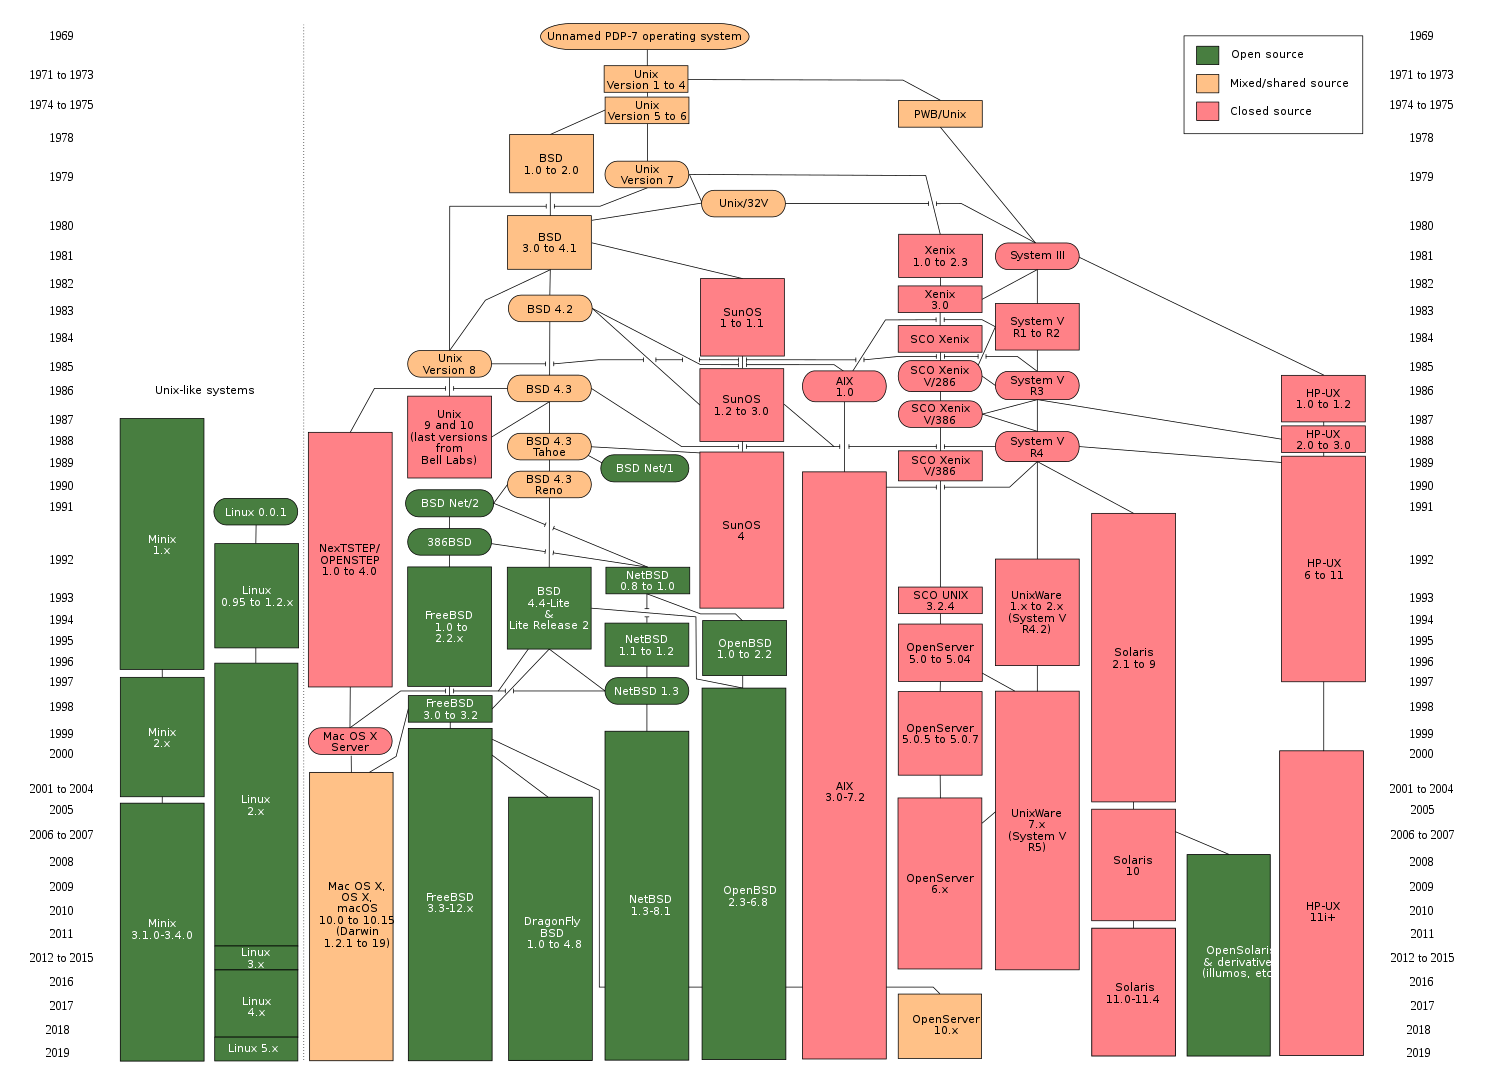
\includegraphics[width=0.75\textwidth]{Unix_history-simple.svg.png}
    \caption{Grafika od Wikimedia Commons}
\end{figure}

Linux nie stanowi produktu jednej firmy, jak np. Windows, jest natomiast wynikiem pracy wielu firm i ogromnej liczby różnych grup ludzi, często działającej na tym polu bezinteresownie (non-profit). GNU/Linux jest bazowym komponentem, na którego podstawie rodzą się inne produkty, nazywane \textbf{dystrybucjami}.

Poszczególne dystrybucje różnią się od siebie mniej lub bardziej wyglądem oraz przeznaczeniem - możemy więc tutaj wybierać pomiędzy dużymi, kompletnymi systemami na domowe biurka, na serwery, do firm a między małymi, lekkimi, a zarazem szybkimi dystrybucjami nadającymi się np. na starsze komputery, czy urządzenia pendrive. Podstawy terminala są jednak niemalże takie same niezależnie od danej dystrybucji. Osobiście piszę ten dokument na dystrybucji o nazwie \say{Fedora}, która \say{utrzymywana} jest przez firmę Red Hat, ale większość komend, (a w szczególności tych z pierwszych rozdziałów) działać będzie również na np. Ubuntu.

% TODO Dodać linki
Jednymi z obecnie najpopularniejszych dystrybucji (w losowej kolejności) są:

\begin{itemize}
    \item Ubuntu
    \item Debian
    \item Linux Mint
    \item Manjaro
    \item Fedora
    \item Pop!\_OS
    \item Elementary
    \item Gentoo
\end{itemize}

Już teraz wiem, że ta lista się dobrze nie zestarzeje. Ponadto proszę o nieinteresowanie się tym ostatnim wymienionym.

Dużą zaletą Linuksów jest to, że jako oparte głównie o wolne oprogramowanie, są one dostępne w większości zupełnie za darmo i to całkiem legalnie. Istnieją oczywiście komercyjne wersje zawierające dodatkowe oprogramowanie, jednakże nawet i one mają konkurencyjne ceny w stosunku do np. oprogramowania Microsoftu. 

\subsection{Co to terminal?}

Bardzo ważną cechą systemów uniksowych jest \textbf{rozdzielenie systemu}, czyli procesów wykonujących zadania, \textbf{od interfejsu}. Dotyczy to nie tylko interfejsu graficznego, ale także i tekstowego.

Jądro Linux ma zaimplementowaną \textbf{emulację terminali}. Historycznie terminale były to komputery o minimalnych możliwościach obliczeniowych i bez własnej pamięci masowej, ale z monitorem i klawiaturą. Za pomocą tych terminali można było sterować główną jednostką obliczeniową. Taki podział był spowodowany m.in. przez bardzo wysoką cenę komputerów w tamtym czasie, i umożliwiał pracę na wielu stanowiskach, z użyciem tylko jednego komputera.

Obecnie wbudowana obsługa terminali w GNU/Linuxie umożliwia zarówno zdalną pracę (np. zdalną administrację serwerem), jak i wykorzystanie wielozadaniowości systemu także w środowisku tekstowym (uruchomienie wielu terminali odpowiada funkcjonalnie otwarciu wielu okien, gdzie w czasie gdy jeden program jest zajęty i nie odpowiada, możemy pracować w innym).

\begin{figure}[H]
    \centering
    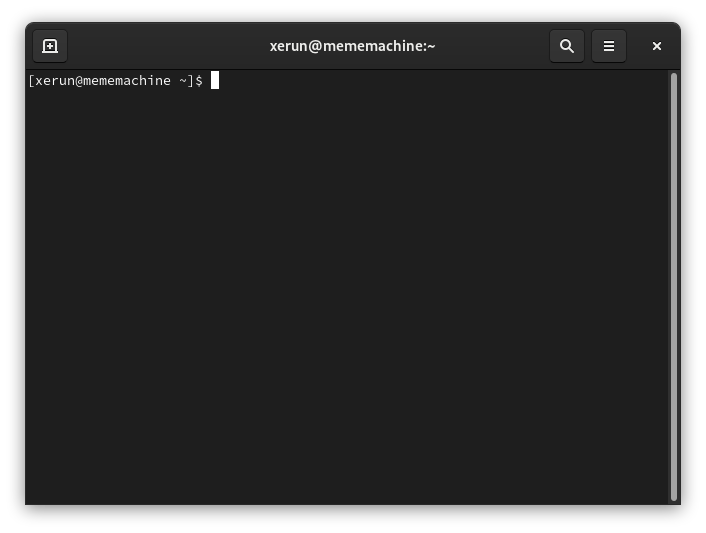
\includegraphics[width=0.75\textwidth]{przyklad terminal.png}
    \caption{Przykład aplikacji emulującej terminal}
\end{figure}

Taka budowa ma również skutki dla twórców oprogramowania - umożliwia to napisanie aplikacji która nie ma praktycznie interfejsu, tylko komunikuje się z użytkownikiem za pomocą wypisywanych linijek tekstu, a użytkownik wpisuje polecenia. 
%Kiedy chcemy mieć aplikację, która wykonuje dokładnie to samo zadanie, ale ma prostszy interfejs, np. wybór wykonywanej akcji z menu, można napisać po prostu nakładkę na nasz pierwotny program, i jego wyjście i wejście przekierować do tej nakładki, zamiast na ekran (czyli terminal). 

\subsection{Co to komendy i polecenia?}

\textbf{Komendy} i \textbf{polecenia} są synonimami. Oznaczają one dowolną instrukcję daną przez użytkownika do systemu, np. uruchomienie programu. Komendy są egzekwowane przez wpisanie ich do linii komend (w terminalu) i naciśnięcie klawisza ENTER.

Warto wiedzieć, że do niemalże każdej komendy na systemie Linux istnieje wbudowana instrukcja obsługi, do której dostać się można za pomocą polecenia:

\ttbf{man \emph{nazwa\_komendy}}

Może się to okazać przydatne, jeśli wyjaśnienie interesującej Cię komendy nie istnieje w tym dokumencie, lub uznasz, że obecne nie jest dla Ciebie wystarczające. Nazwa \ttbf{man} \emph{prawdopodobnie} pochodzi od słowa \say{manual}, ale kto wie tbh, równie dobrze może oznaczać człowieka. Do dziś nie wiadomo do końca co poeta miał na myśli. W moim wypadku instrukcje serwowane są w języku angielskim, na niektórych dystrybucjach jednak istnieje również wersja polska tych tekstów.

\subsection{Uruchamianie terminala}

Zależnie od dystrybucji możecie się spotkać z różnymi nazwami aplikacji emulujących terminal. Aby wam ułatwić znalezienie odpowiedniej aplikacji wypiszę nazwy, pod którymi może się ona kryć:

\begin{itemize}
    \item Terminal
    \item Konsole
    \item Terminator
    \item Yakuake
    \item Kitty
    \item xterm
\end{itemize}

\begin{figure}[H]
    \centering
    \subfloat[Ikony aplikacji 'Terminal']{\includesvg[height=2.5cm]{src_fullcolor_legacy_terminals.svg}}
    \quad
    \subfloat['Konsole']{\includesvg[height=2.5cm]{utilities-terminal.svg}}
    \caption{Przykładowe ikony}
\end{figure}

Po uruchomieniu terminala możecie być słusznie lekko zagubieni. Spotykacie się z jakimiś nazwami w nawiasach, jakimś dolarem i migającym kursorem. Wyjaśnię więc wszystko od początku \dots

Oto przykładowy widok po uruchomieniu aplikacji emulującej terminal na swoim systemie (w moim przypadku to \say{Terminal}):

\begin{console1}

\end{console1}

Oczywiście jest to tylko wersja tekstowa, ale mniej więcej reprezentuje to, co powinniście widzieć. Kolory mogą być inne, a nazwy \ttbf{user} i \ttbf{linux} są definitywnie u was inne.

Zacznę więc od wyjaśnienia od lewej do prawej. To enigmatyczne \ttbf{user} to jesteście \emph{wy}. To wasza nazwa użytkownika i pod tą nazwą znani jesteście dla systemu. Nazwa ta nie zawiera nigdy żadnych dużych liter i zwykle jest też nazwą waszego katalogu domowego (spokojnie, to też wyjaśnię potem).

Następnie widzimy znak \ttbf{@} oraz \ttbf{linux}. To pierwsze po prostu w języku angielskim \say{at} oznacza \say{na}, tymczasem \ttbf{linux} oznacza po prostu nazwę systemu albo komputera, na którym się znajdujecie. W luźnym tłumaczeniu cała fraza \ttbf{user@linux} oznacza \say{użytkownik na tym systemie}

Kolejny symbol to \ttbf{$\sim$}. Jest to aktualny katalog, w którym się znajdujesz, ta część będzie się zmieniać zależnie od tego, jak zmienisz lokalizację - przykładowo:

\ttbf{[user@linux Wideo]\$} albo \ttbf{[user@linux Pobrane]\$}

O zmianie katalogu dowiesz się więcej w następnej sekcji, a konkretnie w "\nameref{sec:cd}"

\ttbf{$\sim$} w systemie Linux oznacza \textbf{katalog domowy} (o czym potem w "\nameref{sec:homedir}")

Fraza zostaje zamknięta w nawiasach i następuje po niej symbol \ttbf{\$}, który można interpretować jako \say{wykonuje}.

Cała fraza oznacza zatem mniej więcej \say{użytkownik na tym komputerze i w tym katalogu wykonuje...}.

\section{Łażenie po świecie - czyli katalogi i pliki}

Należy się przyzwyczaić do myślenia, że obsługując terminal zawsze będziemy w jakimś katalogu. Czy to nasz katalog domowy czy katalog z filmami, nasze działania nie są odizolowane od świata. W tej sekcji przedstawię, jak oddziaływać na ten świat i jak się w nim swobodnie poruszać.

\subsection{Domek czyli \texttt{/home} sweet \texttt{/home}}
\label{sec:homedir}

\textbf{Katalog domowy} to katalog oddzielny dla każdego użytkownika, którego celem jest przechowywanie jego plików i dokumentów (czegokolwiek sobie zapragnie). Katalogi te znajdują się w katalogu \ttbf{/home} (czyli \say{w domku}) i opatrzone są twoją nazwą użytkownika. Przykładowo, będąc zalogowanym jako \ttbf{user}, ścieżka naszego katalogu domowego to \ttbf{/home/user}

Domyślnie, po otwarciu terminala, to w tym katalogu (znanym też jako $\sim$) będziemy się znajdować i w nim rozpoczniemy naszą podróż.

\subsection{Gdzie jestem? - \texttt{pwd}}

Najprostszą komendą, dzięki której nigdy się nie zgubisz, jest \ttbf{pwd} (ang. \textbf{p}rint \textbf{w}orking \textbf{d}irectory)

Jeśli czujecie się zagubieni, nie wiecie gdzie się znajdujecie lub na jakim katalogu operujecie, to ta komenda jest dla was przyjacielem.

\subsubsection{Przykłady}

\begin{enumerate}
    \item \begin{console1}
        pwd
    \end{console1}
    
    \texttt{/home/user}

    \item \ttbf{[user@linux Wideo]\$ pwd}

    \texttt{/home/user/Wideo}
\end{enumerate}

\dots i to wszystko, co ta komenda oferuje tbh.

\subsection{Co jest w moim katalogu? - \texttt{ls} i inne fafarstki}
\label{sec:ls}

Polecenie służące do wypisywania plików i katalogów w danym katalogu. Bez podania żadnych argumentów wypisuje pliki w obecnym katalogu roboczym, czyli tym, w którym się aktualnie znajdujesz. Jedna z najważniejszych komend, jakie można znać na Linuxie.

Komenda nie jest trudna, jej nazwa może też się kojarzyć z angielskim słowem \say{list} czyli wypisywać. Oto składnia:

\ttbf{ls \emph{-opcje} \emph{katalog}}

I jak już wcześniej wspominałem, nie wpisując argumentu \texttt{\emph{katalog}} otrzymamy wynik dla obecnego katalogu roboczego.

Dzięki tej komendzie dowiemy się również, jak wygląda podstawowa struktura katalogu, co w nim jest, jakie są tutaj typy danych i rozwiążemy zagadkę \say{czy katalogi w ogóle istnieją?}

\subsubsection{Niewidoczne rzeczy w katalogach}

Katalogi w systemie Linux mogą zawierać wiele rzeczy, również takich domyślnie niewidocznych dla nas, zwykłych śmiertelników. Zwykle są to pliki konfiguracyjne, lub foldery zawierające takowe, których normalnie nie chcielibyście widzieć, bo tylko wchodzą w drogę, mają jednak wszystkie cechę wspólną - ich nazwa zaczyna się od \say{\ttbf{.}}. Przykładowe pliki i katalogi to: \ttbf{.bashrc}, \ttbf{.cache}, \ttbf{.config}.

Poza wspomnianymi katalogami i plikami konfiguracyjnymi (lub własnymi ukrytymi rzeczami) istnieją stałe 2 nazwy katalogów które należy zapamiętać:
\begin{enumerate}
    \item \ttbf{.} - oznacza aktualny katalog roboczy.
    \item \ttbf{..} - oznacza katalog nadrzędny, \say{wyższy} w hierarchii.
\end{enumerate}

Są to skróty, których celem jest umilenie Ci czasu. Dzięki nim, zamiast wpisywać całą ścieżkę pliku lub katalogu do jakiegoś polecenia, po prostu ich używasz.

Na przykład, jeśli znajdujesz się w katalogu \ttbf{Muzyka}, ale chcesz mieć prostą do wpisania ścieżkę do katalogu \ttbf{Wideo}, który znajduje się w katalogu nadrzędnym, to w tym wypadku ścieżka do niego wygląda tak: \ttbf{../Wideo}

Łatwiej jest to sobie zwizualizować mając drzewko hierarchii folderów:

\dirtree{%
    .1 home.
    .2 user.
    .3 CLionProjects.
    .3 Dokumenty.
    .3 GOG Games.
    .3 MultiMC.
    .3 Muzyka.
    .4 \textbf{(Tu jesteś)}.
    .3 Obrazy.
    .3 Pobrane.
    .3 Publiczny.
    .3 Pulpit.
    .3 PycharmProjects.
    .3 Szablony.
    .3 Wideo.
    .4 \textbf{(Tu chcesz coś zrobić)}.
}\hfill

Komenda \say{\ttbf{ls .}} będzie robić dokładnie to samo co zwykła komenda \say{\ttbf{ls}}. Po prostu w tym drugim wypadku program się domyśla, że chodzi o kropkę.

\subsubsection{Opcje}
\begin{itemize}
    \item \texttt{a} (all) Wypisuje \emph{wszystkie} elementy w katalogu, nawet te ukryte.
    \item \texttt{l} (long) Wypisuje dodatkowe dane w kolumnach (uprawnienia, ilość dowiązań, właściciela, grupę, do której należy plik/katalog, rozmiar, datę modyfikacji, nazwę pliku).
    \item \texttt{h} (human-readable) Pokazuje jednostki bardziej czytelne dla ludzi (np. 2M(egabajty), 1G(igabajt)).
    \item \texttt{S} (sort by Size) Sortuje wynik po rozmiarze (największy pierwszy).
    \item \texttt{t} (sort by time) Sortuje wynik po czasie (najnowszy pierwszy).
\end{itemize}

Komendy można łączyć ze sobą jednocześnie, np. \ttbf{-al} wypisuje wszystkie, nawet ukryte, elementy w kolumnach razem z dodatkowymi danymi. Kolejność nie ma znaczenia, \ttbf{-al} robi dokładnie to samo co \ttbf{-la}

\subsubsection{Przykłady}
\begin{enumerate}

    \item Proste wykonanie:

    \begin{console1}
    ls
\end{console1}

\begin{verbatim}
CLionProjects  'GOG Games'   Muzyka   Pobrane     Pulpit            Szablony
Dokumenty       MultiMC      Obrazy   Publiczny   PycharmProjects   Wideo
\end{verbatim}

Jak wydać powyżej, polecenie \ttbf{ls} wypisuje każdy nieukryty element w katalogu roboczym. Sortowane są one alfabetycznie po nazwie, niezależnie od typu (plik/katalog/coś innego). Elementy, których nazwy są wieloczłonowe są opatrzone w cudzysłowie, żeby ich przypadkowo nie wziąć za oddzielne elementy.

\item Wyświetlanie jako lista:

\begin{console1}
    ls -l
\end{console1}

\begin{verbatim}
razem 48
drwxr-xr-x. 7 user user 4096 01-14 00:16  CLionProjects
drwxr-xr-x. 6 user user 4096 01-30 13:33  Dokumenty
drwx------. 3 user user 4096 08-19 23:49 'GOG Games'
drwxr-xr-x. 5 user user 4096 01-11 23:24  MultiMC
drwxr-xr-x. 2 user user 4096 08-15 15:59  Muzyka
drwxr-xr-x. 4 user user 4096 01-30 18:21  Obrazy
drwxr-xr-x. 2 user user 4096 02-14 00:15  Pobrane
drwxr-xr-x. 2 user user 4096 08-15 15:59  Publiczny
drwxr-xr-x. 3 user user 4096 02-13 14:19  Pulpit
drwxr-xr-x. 3 user user 4096 11-18 14:14  PycharmProjects
drwxr-xr-x. 2 user user 4096 08-15 15:59  Szablony
drwxr-xr-x. 6 user user 4096 02-13 18:38  Wideo
\end{verbatim}

\item Wyświetlenie posortowanej po rozmiarze listy elementów z katalogu Wideo:

\begin{console1}
    ls -lhS Wideo
\end{console1}

\begin{verbatim}
razem 238M
-rw-r--r--. 1 user user  71M 12-09 05:34  projekt2hq.mp4
-rw-r--r--. 1 user user  30M 02-08 18:17 '2021-02-08 18-05-21.mkv'
-rw-r--r--. 1 user user  30M 12-09 05:23  projekt2.mp4
-rw-r--r--. 1 user user  19M 02-03 00:52 '2021-02-03 00-45-41.mkv'
-rw-r--r--. 1 user user 180K 02-03 00:45 '2021-02-03 00-45-01.mkv'
-rw-r--r--. 1 user user  65K 01-15 22:09  projekt3.kdenlive
drwxrwxr-x. 2 user user 4,0K 02-13 18:38  Film
drwxr-xr-x. 2 user user 4,0K 02-08 19:11 'Projekt 3'
drwxr-xr-x. 2 user user 4,0K 01-15 22:04  Projekt2
drwxr-xr-x. 2 user user 4,0K 01-15 21:51  titles
\end{verbatim}
\end{enumerate}

\subsection{Zmiana katalogu - \texttt{cd}}
\label{sec:cd}

To najważniejsza komenda w tej całej sekcji. Dzięki niej zrobisz wszystko i nic.

\ttbf{cd}, czyli \textbf{c}hange \textbf{d}irectory, to polecenie służące do przemieszczania się między folderami. Poniżej składnia komendy:

\ttbf{cd \emph{katalog}}

Dodatkowo istnieją pewnie stałe nazwy, które są powtarzalne i obecne w każdym folderze:

\begin{itemize}
    \item \ttbf{..} - aby wejść do katalogu \emph{wyższego} w hierarchii, czyli np. z \ttbf{/Wideo/Filmy} do \ttbf{/Wideo}, zamiast wpisywać całą ścieżkę możemy zastąpić ją tymi dwoma kropkami (\ttbf{cd ..})
    \item \ttbf{.} - oznacza obecny katalog. Dużo z tym nie zrobimy, bo zmiana katalogu na obecny nie ma za bardzo sensu, ale jest przydatne z innych powodów, o których się dowiesz \textbf{potem}.
\end{itemize}

\subsubsection{Przykłady}

Zakładając, że wasz katalog domowy wygląda tak po wpisaniu komendy \hyperref[sec:ls]{\ttbf{ls}}:

\begin{verbatim}
CLionProjects  'GOG Games'   Muzyka   Pobrane     Pulpit            Szablony
Dokumenty       MultiMC      Obrazy   Publiczny   PycharmProjects   Wideo
\end{verbatim}

Jeśli chcemy wejść do katalogu Wideo, możemy wpisać:

\begin{console1}
    cd Wideo
\end{console1}

albo

\begin{console1}
    cd /home/user/Wideo
\end{console1}

Dodatkowo po wpisaniu:

\ttbf{[user@linux Wideo]\$ cd ..}

wrócimy do katalogu \emph{wyżej} (czyli w tym wypadku $\sim$).

\end{document}
